\documentclass[utf8,hyperref={colorlinks=true}]{beamer}
\definecolor{links}{HTML}{2A1B81}
\hypersetup{colorlinks,linkcolor=,urlcolor=links}
\mode<presentation>
\usepackage{listings}
\usepackage{helvet}
\usetheme{Frankfurt}
\usecolortheme{whale}
\usefonttheme[onlylarge]{structuresmallcapsserif}
\usefonttheme[onlysmall]{structurebold}
\usepackage{amsthm} % pushQED, popQED
\newenvironment{aquote}[1]{%
  \pushQED{#1}%
  \begin{quote}
}{%
  \par\noindent\hfill(\popQED)%
  \end{quote}%
}

\setbeamercovered{dynamic}
\setbeameroption{show notes}

\begin{document}
\title{The Lucene Server}
\subtitle{A bridge between two worlds}
\author{Fernando Benavides (\textit{@elbrujohalcon})}
\institute{Inaka Labs}
\date{\today}
\logo{
\includegraphics[height=0.5cm]{img/inaka_leaf_logo.png}}

\newcommand*\oldmacro{}%
\let\oldmacro\insertshorttitle%
\renewcommand*\insertshorttitle{%
  \oldmacro\hfill%
  \insertframenumber\,/\,\inserttotalframenumber}

%%%%%%%%%%%%%%%%%%%%%%%%%%%%%%%%%%%%%%%%%%%%%%%%%%%%%%%%%%%%%%%%%%%%%%
%% CODE SNIPPETS
%%%%%%%%%%%%%%%%%%%%%%%%%%%%%%%%%%%%%%%%%%%%%%%%%%%%%%%%%%%%%%%%%%%%%%
\definecolor{darkblue}{rgb}{0,0.08,0.45} 

\lstset{% general command to set parameter(s)
		mathescape=true,
		language=erlang,
		basicstyle=\ttfamily\small,
		keywordstyle=\color{blue}\bfseries,
		identifierstyle=\color{darkblue},
		stringstyle=\ttfamily,
		showstringspaces=false}

\defverbatim[colored]\startchild{%
\begin{lstlisting}[frame=single]
start_user(User) ->
  Manager =
    list_to_atom(
      "user-manager-" ++
        integer_to_list($\colorbox{yellow}{\texttt{random:uniform(?MANAGERS)}}$)),
  supervisor:start_child(Manager, [User]).
\end{lstlisting}
}

%%%%%%%%%%%%%%%%%%%%%%%%%%%%%%%%%%%%%%%%%%%%%%%%%%%%%%%%%%%%%%%%%%%%%%

\frame{\titlepage} 

\section{Introduction}
\subsection{Description}
\begin{frame}{TigerText}
	\begin{aquote}{from\href{http://http://www.tigertext.com/}{TigerText Site}}
	TigerText is a secure mobile messaging platform that you set up for your hospital or business to improve workflow and reduce risk. Employees gain the convenience and familiarity of traditional texting while the enterprise retains the control and security it demands.
	\end{aquote}
\end{frame}
\begin{frame}{Autocomplete}
	\emph{They wanted this\ldots}
	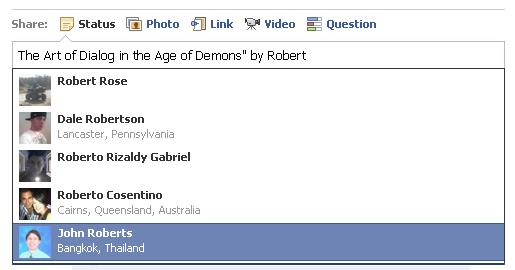
\includegraphics[width=\textwidth]{img/autocomplete.jpeg}
\end{frame}
\subsection{Scope}
\begin{frame}{Scope}
	\emph{The goals for this talk are to show you:}
	\begin{itemize}
		\item how we connected two seemingly icompatible worlds
		\item how we started with a very specific problem and ended up with a very general solution
	\end{itemize}
\end{frame}

\section{The Project}
\subsection{The Story}
\begin{frame}{The Problem}
	\only<1>{\emph{Once upon a time on server world\ldots}}
	\only<2>{\emph{Erlang} and \emph{Redis} were happily talking}
	\only<3>{But they needed \emph{Lucene}, something that only \emph{Java} knew\ldots}
	\only<4>{\ldots and \emph{Java}, well\ldots}
	\begin{center}
		\includegraphics<1-3>[]{img/talking.jpeg}
		\includegraphics<4>[width=\textwidth]{img/not-talking.jpeg}
	\end{center}
\end{frame}

\subsection{Our Work}
\begin{frame}
	\only<1>{\emph{Oh! Now who can help?!}\footnote{Translated by $Google^{TM}$}}
	\begin{flushright}
	\only<2>{\emph{Yo! The red locust! They did not have my cunning!}\footnote{Translated by $Google^{TM}$}}
	\end{flushright}
	\begin{center}
	\only<3>{\emph{\ldots ehm\ldots that would be \textbf{us}}}
	\end{center}
	\begin{center}
		\includegraphics<1>[height=.5\textheight]{img/distress.jpeg}
		\includegraphics<2>[height=.75\textheight]{img/chapulin.jpeg}
		\includegraphics<3>[height=.75\textheight]{img/inaka.png}
	\end{center}
\end{frame}

\subsection{Tools}
\begin{frame}{JInterface}
	\begin{aquote}{from\href{http://www.erlang.org/doc/man/jinterface.html}{Erlang Docs}}
	Jinterface Java package contains java classes, which help you integrate programs written in Java with Erlang
	\end{aquote}
\end{frame}
\begin{frame}{JInterface}
	\begin{itemize}
		\item<+->Comes with the Erlang distribution
		\item<+->Is written in Java
		\item<+->Lets you create nodes and processes inside a Java VM
		\item<+->\emph{We extended it to handle OTP \textit{gen\_server} protocol}
	\end{itemize}
\end{frame}
\begin{frame}{Lucene}
	\begin{aquote}{from \href{http://lucene.apache.org/}{Lucene Site}}
	Apache Lucene$^{TM}$ is a high-performance, full-featured text search engine library written entirely in Java. It is a technology suitable for nearly any application that requires full-text search, especially cross-platform.
	\end{aquote}
\end{frame}
\begin{frame}{Lucene}
	\begin{itemize}
		\item<+->It lets us work with documents that represent users
		\item<+->It analyzes, tokenizes and indexes the different fields
		\item<+->\emph{Using it together with JInterface, we built a Java \textit{node} with a Lucene-backed Autocomplete \textit{gen\_server}}
	\end{itemize}
\end{frame}

\subsection{Conclusions}
\begin{frame}{What we've found?}
	\begin{itemize}
		\item<+->Processing is fast, communications are slow
		\item<+->Lucene is not complete, but it's really flexible
		\item<+->JInterface is very basic, not exactly flexible, but in fact extensible
	\end{itemize}
\end{frame}

\section{Last Words}
\subsection{Generalizing}
\begin{frame}{Generalizing}
	\begin{itemize}
		\item<+->Now that we have it, we can use Lucene in other Erlang applications
		\item<+->We've split Autocomplete from Lucene logic
		\item<+->Then we've created a Lucene Server for Erlang
		\item<+->It's still in its early stages, there's a lot to improve on that
	\end{itemize}
\end{frame}

\begin{frame}{Resources}
	\begin{description}
		\item[About me]~\\
			\begin{itemize}
				\item I'm \textbf{\href{http://twitter.com/elbrujohalcon}{@elbrujohalcon}} at Twitter
				\item I'm \href{http://github.com/elbrujohalcon}{elbrujohalcon} at Github
			\end{itemize}
		\item[About Inaka]~\\
			\begin{itemize}
				\item Check our website: \href{http://inakanetworks.com}{http://inaka.net}
				\item And our Blog that's on the same site
			\end{itemize}
		\item[About This Talk]~\\
			\begin{itemize}
				\item This talk is on Github: \href{http://github.com/inaka/talks/pdfs/lucene\_server.pdf}{http://github.com/inaka/talks}
			\end{itemize}
	\end{description}
\end{frame}

\appendix

\begin{frame}
	\begin{center}
		{\Huge Thanks!}
	\end{center}
\end{frame}

\end{document}